\graphicspath{{fig/}}

\chapter{Methodology}
\label{chap:method}

%  A paragraph Outling what is discussed in this chapter from a high level perspective. The Core hypotheis is repeated concisesly. Using the hypothesis as a source this high-level pipeline is briefly described. The 


The preceding chapters established that while contrastive learning successfully structures feature spaces and model performance is correlated with desirable weight space geometry, a comprehensive framework uniting these two domains remains elusive. This chapter introduces our core methodological contribution: a novel **Contrastive Weight Space Learning** framework designed to create a unified latent space for network weights, dataset characteristics, and resultant performance metrics.

% The user's existing high-level description is integrated here:
In this report, we develop a contrastive learning framework to create a unified embedding space that jointly represents network weights ($\mathcal{W}$), the datasets they were trained on ($\mathcal{D}$), and their resulting performance characteristics ($\mathcal{R}$). Specifically, we construct two separate encoders—one for dataset embeddings using pre-trained CLIP features, and another for weight embeddings using an autoencoder architecture—alongside a binned result embedding table. These encoders are trained using the contrastive objective NT-Xent \cite{agren2022ntxentlossupperbound}, which encourages related triplets $(\mathcal{D}, \mathcal{W}, \mathcal{R})$ to be close in the shared latent space. Figure \ref{fig:pipeline_2} depicts a high-level view of the full embedding pipeline.

\begin{figure}[!t]
    \centering
    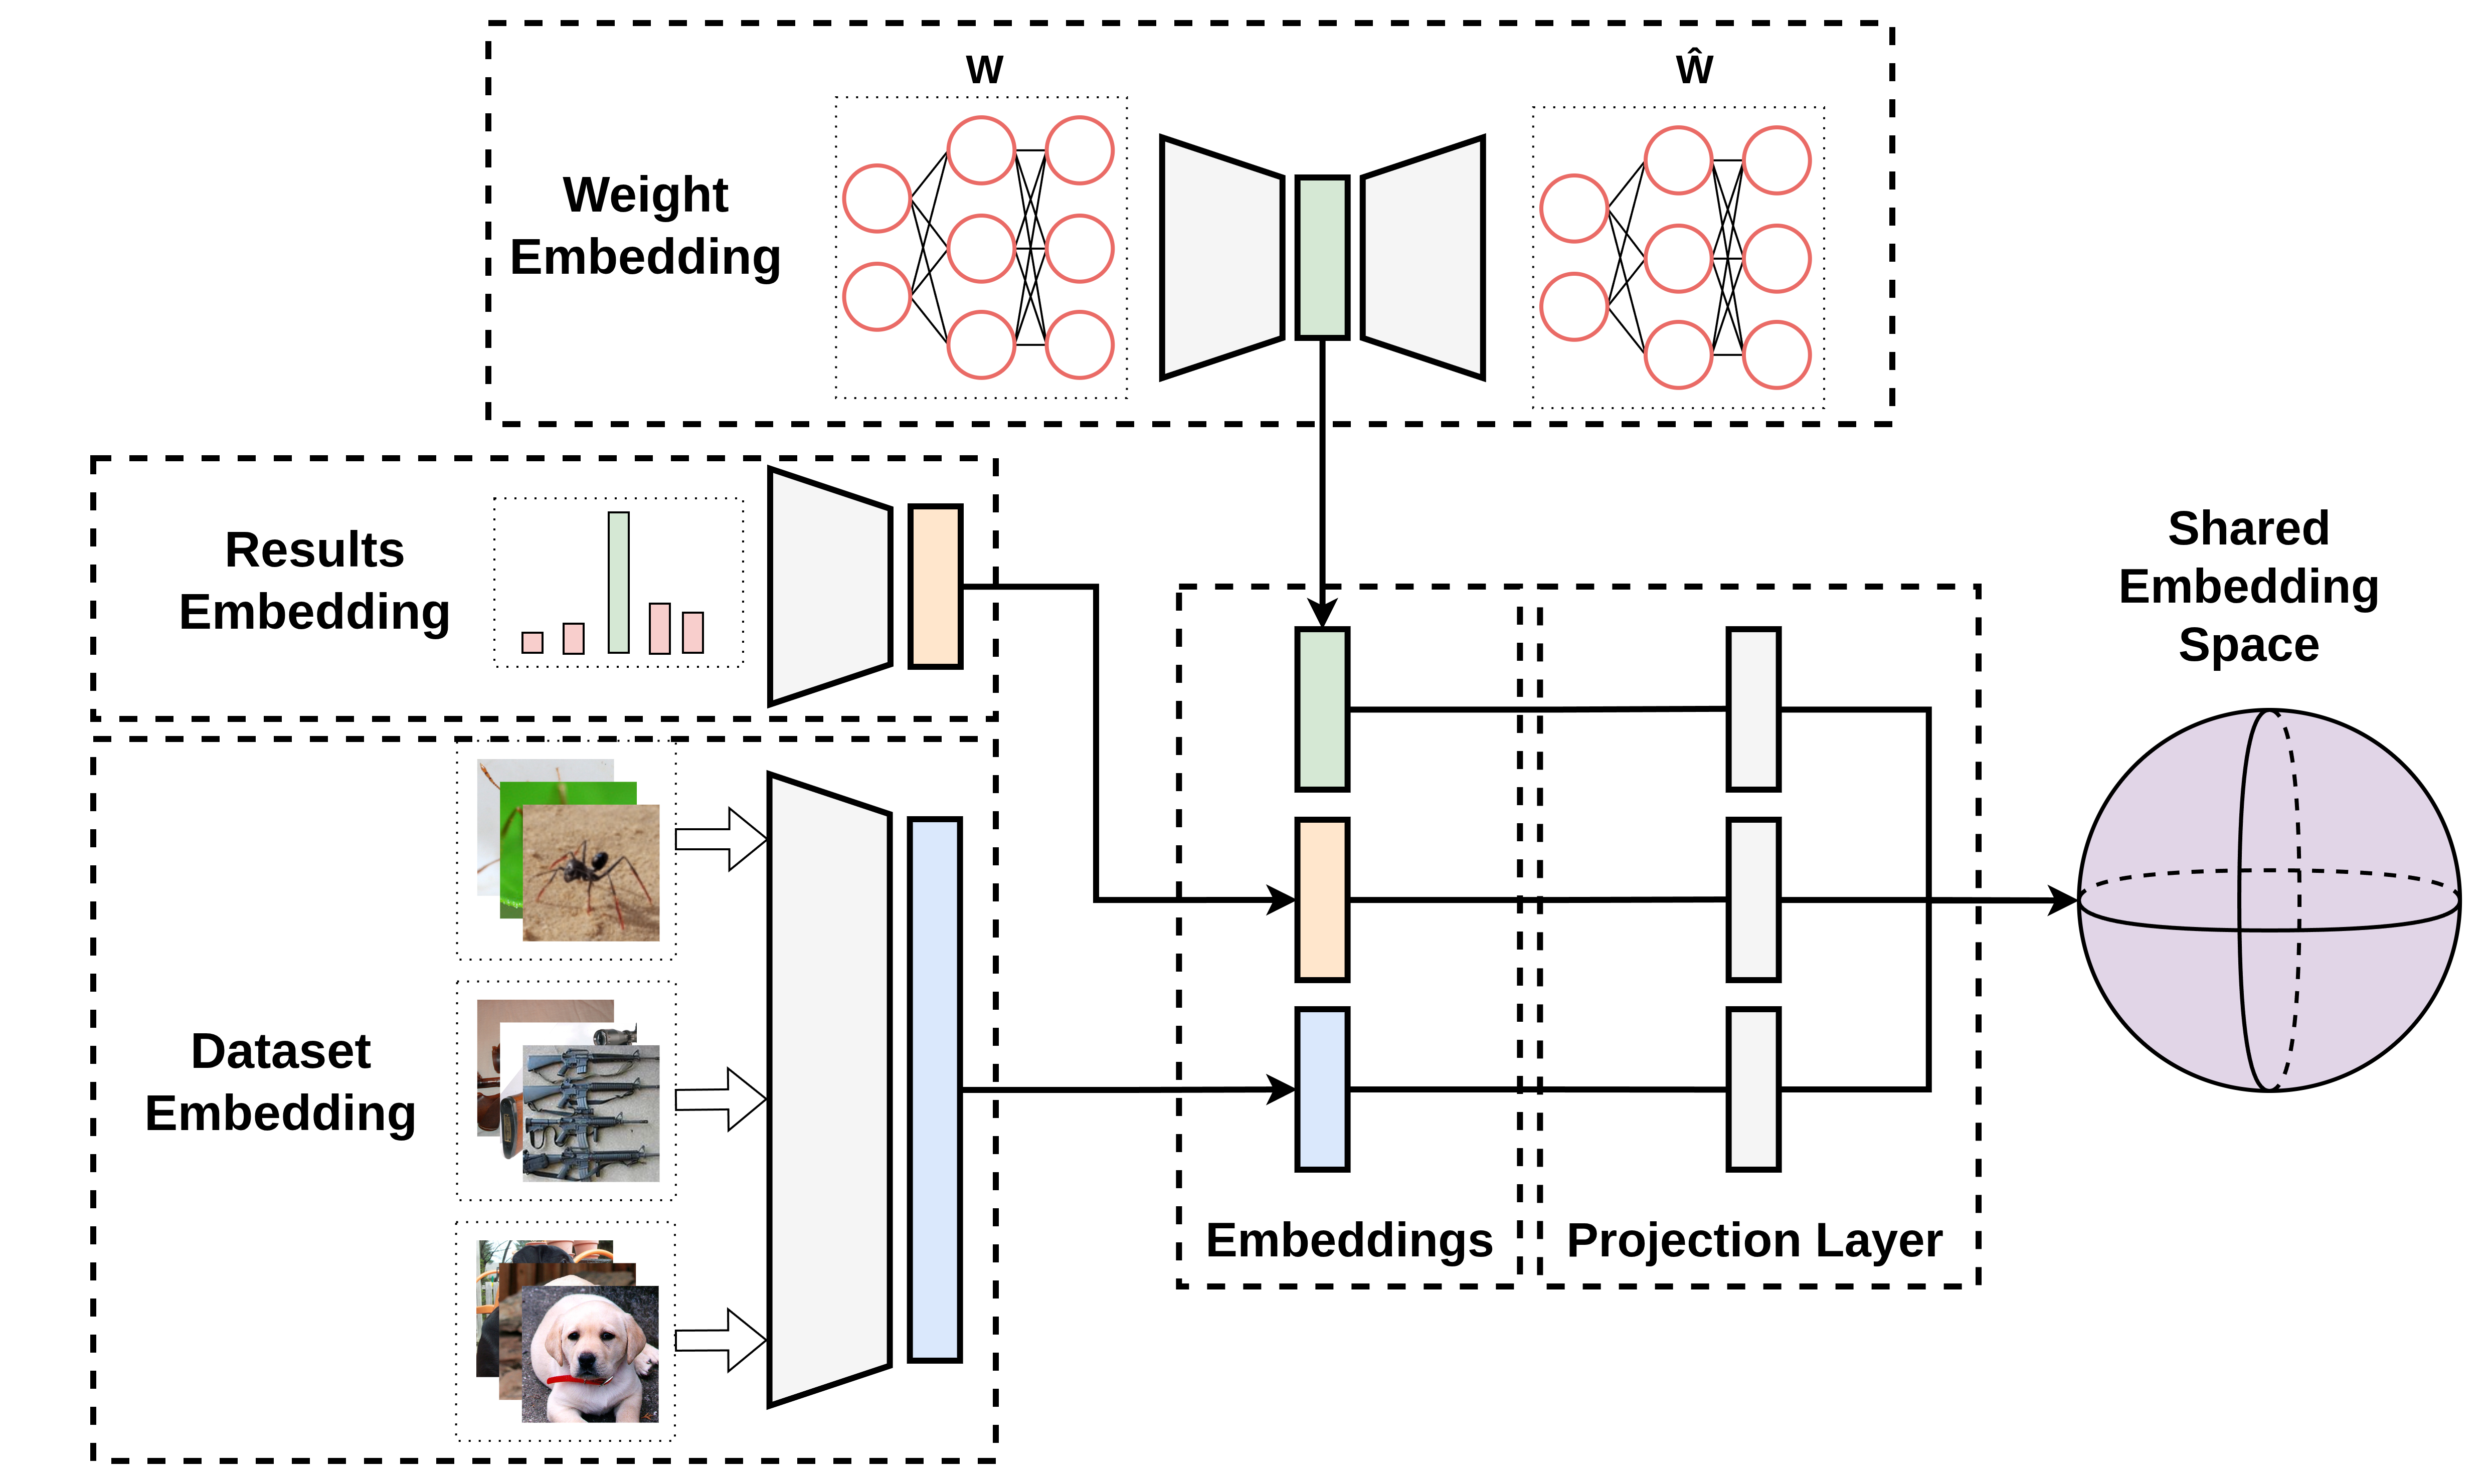
\includegraphics[width=0.75\linewidth]{pipeline.png}
    \caption[A figure illustrating the process of embedding a dataset, model weigths and results into a shared embedding space ]{A figure illustrating the process of embedding a dataset, model weights and results in a shared embedding space. }
    \label{fig:pipeline_2}
\end{figure}

The success of this framework relies on solving several key representation and alignment problems. The rest of this chapter is structured to systematically address these challenges, moving from the generation of the raw input data to the final unified training objective.

First, Section \ref{sec:data_gen} outlines the essential problem of **Data Generation**, detailing the process of curating a large, diverse collection of $(\mathcal{D}, \mathcal{W}, \mathcal{R})$ triplets, specifying the model architectures (e.g., ResNet18), dataset types (e.g., subsets of Imagenet), optimization parameters, and hyperparameter ranges necessary to ensure the captured weight-result space is rich and varied.

Next, we address the challenge of representing each component in an efficient, meaningful manner. Section \ref{sec:weight_enc} discusses the design and rationale for the **Weight Encoder**, which must compress the extremely high-dimensional, ordered weight tensor ($\mathcal{W}$) into a fixed-size latent vector while preserving critical information about the weight configuration's geometric properties.

The representation of the input context is tackled in Section \ref{sec:data_enc}, which explains the **Dataset Encoder** leveraging CLIP features to transform datasets ($\mathcal{D}$) into a semantic embedding that captures the visual and conceptual characteristics of the training data.

Section \ref{sec:results_enc} then details the **Results Encoder**, clarifying how the scalar performance metrics ($\mathcal{R}$) are quantized and embedded into a fixed-size vector, providing a discrete target representation for the contrastive objective.

Finally, Section \ref{sec:shared_enc} integrates these components by explaining the **Shared Encoding** framework. This section details the application of the NT-Xent loss to align the three distinct embeddings—dataset, weight, and result—into a single, unified latent space, defining the optimization objectives and the final training schedule.


\section{Data Generation}
\label{sec:data_gen}
ResNet18
Imagenet
optimisation
Hyperparemeter range 

Traqining Schedule explanation
Sample Size justification

\section{Weight Encoder}
\label{sec:weight_enc}
What we need:

What is available

What was used and why
SAN, referenced Background performs

\section{Dataset Encoder}
\label{sec:data_enc}

CLIP
Feature exsstractions, and then average over all training images of a class
\section{Results Encoder}
\label{sec:results_enc}
\section{Shared Encoding}
\label{sec:shared_enc}
